
%%%%%%%%%%%%%%%%%%%%%
\chapter{Fonctions initiales}
%%%%%%%%%%%%%%%%%%%%%

%%%%%%%%%%%%%%%%%%%%%
\section{Fonctions périodiques}
%%%%%%%%%%%%%%%%%%%%%
\subsection{Définitions}
%%%%%%%%%%%%%%%%%%%%%
i est un entier tel que 0 $\leqslant$ i $<$ N. $\mc{F}_\mt{P}$(i) est une fonction périodique de période P et d'amplitude A. La période peut s'écrire comme la somme d'une puissance de deux ($2^\eta$)
et d'un nombre décimal $\rho$ inférieur à $2^\eta$ :
\[
\mt{P}=2^\eta+\rho\qquad\mt{avec}\qquad\rho<2^\eta
\]

$\mc{M}$(j) est un motif de $\mc{F}_\mt{P}$(i). C'est une fonction de P
points. d est le décalage suivant i de $\mc{F}_\mt{P}$ par rapport à $\mc{M}$.

La fonction périodique $\mc{F}_\mt{P}$(i) peut alors s'écrire :
\[
\mc{F}_\mt{P}\mt{(i)}=\mc{M}\big(\mt{ (i}+\mt{d) modulo P }\big)
\]

%%%%%%%%%%%%%%%%%%%%%
\subsection{Fonction en dent de scie}
%%%%%%%%%%%%%%%%%%%%%

\subsubsection{Moyenne nulle}


\begin{center} 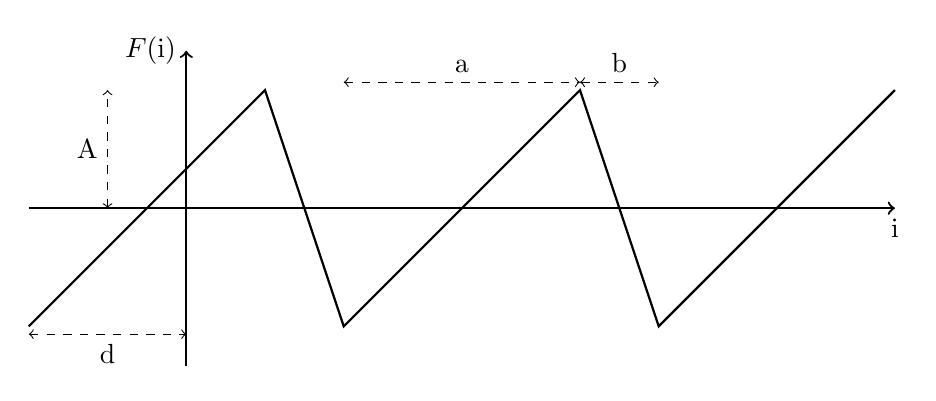
\begin{tikzpicture}
\def \Amp{1.5}
% Axes
\draw [thick, ->] (0,-2) -- (0,2) node [left] {$\mc{F}$(i)};
\draw [thick, ->] (-2,0) -- (9,0) node [below] {i};
% F(x)
\draw [thick] (-2,-\Amp) -- (1,\Amp) -- (2,-\Amp) -- (5,\Amp) -- (6,-\Amp) --(9,\Amp);
% Mesures
\draw [dashed, <->] (2,\Amp+0.1) -- (5,\Amp+0.1); \draw (3.5,\Amp+0.1) node [above] {a};
\draw [dashed, <->] (5,\Amp+0.1) -- (6,\Amp+0.1); \draw (5.5,\Amp+0.1) node [above] {b};
\draw [dashed, <->] (-2,-\Amp-0.1) -- (0,-\Amp-0.1); \draw (-1,-\Amp-0.1) node [below] {d};
\draw [dashed, <->] (-1,0) -- (-1,1.5); \draw (-1,0.75) node [left] {A};
\end{tikzpicture} \end{center}

\begin{minipage}[c]{.45\linewidth}
\begin{center}
j $\in$ $\big[$ 0 , a$+$b $\big[$
\end{center}
\[
\left\{ \begin{array}{rcll}
\mc{M}(\mt{j}) & = & \frac{2\mt{A}}{\mt{a}}\mt{ j}-\mt{A} & \qquad\mt{si j}<\mt{a} \\
\mc{M}(\mt{j}) & = & 2\mt{A}\frac{\mt{a}}{\mt{b}}\mt{ j}-\mt{A}(1-2\frac{a}{b}) & \qquad\mt{si j}>\mt{a} \end{array} \right.
\]
\end{minipage}
\hfill
\begin{minipage}[c]{.45\linewidth}
\begin{center}
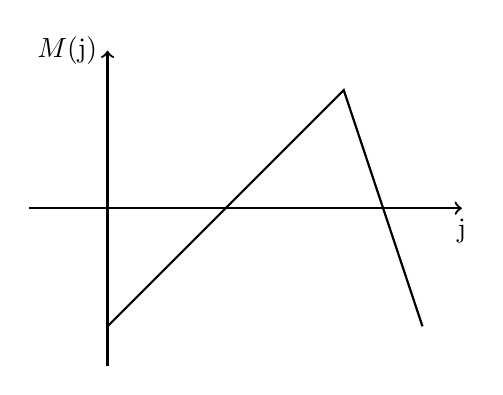
\begin{tikzpicture}
\def \Amp{1.5}
% Axes
\draw [thick, ->] (0,-2) -- (0,2) node [left] {$\mc{M}$(j)};
\draw [thick, ->] (-1,0) -- (4.5,0) node [below] {j}; 
% M(x)
\draw [thick] (0,-\Amp) -- (3,\Amp) -- (4,-\Amp);
\end{tikzpicture} \end{center}
\end{minipage}

\subsubsection{Moyenne non nulle}
$\mc{M}(\mt{j})=\mc{M}(\mt{j})+\mt{B}$

%%%%%%%%%%%%%%%%%%%%%
\subsection{Fonction en créneaux}
%%%%%%%%%%%%%%%%%%%%%

\subsubsection{Moyenne nulle}

\begin{center} \begin{tikzpicture}
\def \Amp{1.5}
% Axes
\draw [thick, ->] (0,-2) -- (0,2) node [left] {$\mc{F}$(i)};
\draw [thick, ->] (-2,0) -- (12,0) node [below] {i};
% F(x)
\draw [thick] (-1,\Amp) -- (1,\Amp);
\draw [thick] (1,-\Amp) -- (4,-\Amp);
\draw [thick] (4,\Amp) -- (6,\Amp);
\draw [thick] (6,-\Amp) -- (9,-\Amp);
\draw [thick] (9,\Amp) -- (11,\Amp);
% Mesures
\draw [dashed, <->] (4,\Amp/2) -- (6,\Amp/2); \draw (5,\Amp/2) node [above] {a};
\draw [dashed, <->] (6,\Amp/2) -- (9,\Amp/2); \draw (7.5,\Amp/2) node [above] {b};
\draw [dashed, <->] (-1,-\Amp/2) -- (0,-\Amp/2); \draw (-0.5,-\Amp/2) node [below] {d};
\end{tikzpicture} \end{center}

\begin{minipage}[c]{.45\linewidth}
\begin{center}
j $\in$ $\big[$ 0 , a+b $\big[$
\end{center}
\[
\left\{ \begin{array}{rcll}
\mc{M}(\mt{j}) & = & \mt{A} & \qquad\mt{si j}<\mt{a} \\
\mc{M}(\mt{j}) & = & -\mt{A} & \qquad\mt{si j}>\mt{a} \end{array} \right.
\]
\end{minipage}
\hfill
\begin{minipage}[c]{.45\linewidth}
\begin{center}
\begin{tikzpicture}
\def \Amp{1.5}
% axes
\draw [thick, ->] (0,-2) -- (0,2) node [left] {$\mc{M}$(j)};
\draw [thick, ->] (-1,0) -- (5.5,0) node [below] {j}; 
% M(x)
\draw [thick] (0,\Amp) -- (2,\Amp);
\draw [thick] (2,-\Amp) -- (5,-\Amp);
\end{tikzpicture} \end{center}
\end{minipage}

\subsubsection{Moyenne non nulle}
$\mc{M}(\mt{j})=\mc{M}(\mt{j})+\mt{B}$

%%%%%%%%%%%%%%%%%%%%%
\section{Fonction en cloche}
%%%%%%%%%%%%%%%%%%%%%
\subsection{Gaussienne}
%%%%%%%%%%%%%%%%%%%%%
\[
\mc{F}\mt{(i)}=\frac{1}{\sigma\sqrt{2\pi}}\mt{ e}^{-\frac{(\mt{i}-\mt{d})^2}{2\sigma^2}}
\]
%%%%%%%%%%%%%%%%%%%%%
\subsection{Lorentzienne}
%%%%%%%%%%%%%%%%%%%%%
\[
\mc{F}\mt{(i)}=\frac{\frac{2}{\pi\Gamma}}{1+\left(\frac{\mt{i}-\mt{d}}{\Gamma/2}\right)^2}
\]




%%%%%%%%%%%%%%%%%%%%%%%%%%%%
